\section{Theory}

	Transverse waves are those where the direction of oscillation is perpendicular to the direction of the propagation wave. Polarization is a property of transverse waves whereby the direction of these oscillations is limited to a particular orientation as shown in the \hyperref[fig:1]{Figure 1}. When the wave is passed, certain materials block the vibrations in certain orientations of an unpolarized transverse wave or retards them concerning other orientations, producing a different state of polarization. Light is a transverse electromagnetic wave consisting of the coupled oscillating electric and magnetic fields which are always perpendicular to each other. By convention, the "polarization" of electromagnetic waves refers to the direction of the electric field. Light is said to be unpolarized when its state of polarization changes more rapidly than it can be detected such that polarization averages out in all directions.
	\begin{figure}[H]
		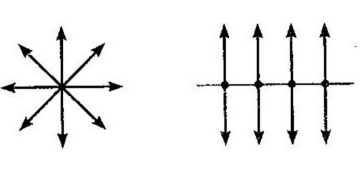
\includegraphics[height=3.5cm, width=7cm]{OPT100.png}
		\caption{Unpolarized (left) and Polarized Light Beam (right)}
		\label{fig:1}
	\end{figure}

	% \vspace{-1cm}
	\subsection{Linearly Polarized Light}

		When a beam of unpolarized light is incident on a polarizer made of a birefringent material, the transmitted beam is polarized in the direction of its transmission axis. Since an unpolarized light can be substituted with two perpendicular but incoherent vibrations, the intensity of the linearly polarized light is halved ( $\sfrac{I_0}{2}$ for intensity $I_0$) as one of the vibrational axis is blocked. Any rotation of the polarizer changes the orientation of the linearly polarized light but not its intensity. \\

		% \vspace{-3mm}
		An ideal linear polarizer has $100\%$ transmission for a linearly polarized light for an orientation parallel to its transmission axis and zero transmission at an orientation orthogonal to it. The transmission relation with the angle difference of the transmission and polarization axis is given by Malu's law. According to Malu's law:
		
		% \vspace{-2mm}
		\begin{equation}
			I= I_0 \cos^2{\theta}
			\label{eqn:1}
		\end{equation}
		
		%\vspace{-1mm}
		where $\theta$ is the angle between between the incident linear polarization and the transmission axis. $I_0$ is the intensity of the linearly polarized light before transmission (or for $\theta=0\degree$) and $I$ is the intensity of the transmitted (rotated) beam. \\

		\vspace{-3mm}
		For verifying Malu's law, we will be using an identical polarizer called an analyzer which will rotate the linearly polarized light coming from the polarizer and by rotating it at an angle with respect to the polarizer's transmission axis. The intensity of transmitted light can be noted using a detector which produces a propotional current in the multimeter.

	%\vspace{-2mm}
	\subsection{Wave Plates (Retarders)}

		Ideal wave plates modify polarization without attenuating or displacing the beam. They retard a particular component of polarization with respect to its orthogonal component. It divides the incident beam into two rays:  one follows the laws of refraction, called the ordinary ray and the other one is called extra-ordinary ray which does not obey the laws of refraction. This is because they have different refractive indices along two perpendicular axes. The refractive indices for the two rays are different which produces a phase difference between the rays given by:
		$$ \psi = \frac{2\pi}{\lambda}(n_o\,-\,n_e)d$$
		where $n_o$ and $n_e$ are refractive index of the ordinary and extra-ordinary rays respectively. $d$ is the thickness and $\lambda$ is the wavelength of the laser beam. Therefore the two perpendicular oscillations form a two perpendicular simple harmonic oscillator system oscillating at a phase difference depending on the wave plate used. 

		\begin{itemize}
			\item \textbf{Half wave plate:}\\
			A retarder is called a half wave plate when causes the phase difference between the two emergent beams to be $\pi$. Therefore a linearly polarized incident at an angle $\theta$ with respect to the fast axis will have its polarization axis rotated by an angle $2\theta$, since now the perpendicular component of the light with respect to the fast axis will be at phase difference of $\pi$ as shown in figure  $\ref{fig2}$.
			%\vspace{-5mm}
			\begin{figure}[H]
				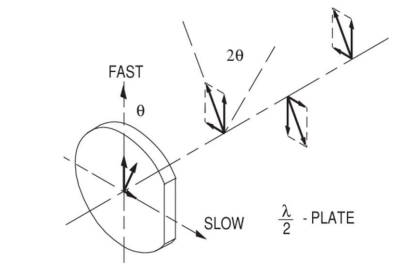
\includegraphics[height=4cm, width=7cm]{OPT1000.png}
				\caption{\textbf{Half Wave Plate rotating a linearly polarized light beam}}
				\label{fig2}
			\end{figure} 

			\item \textbf{Quarter wave plate:}\\
			When the wave plate produces a phase difference of $\frac{\pi}{2}$, it is called a quarter wave plate. The emergent light beam will have circular polarization if the angle between the polarization axis of the linearly polarized light is at an angle of $45\degree$, otherwise it will be elliptically polarized as shown in figure $\ref{fig3}$.
			%\vspace{-4mm}
			\begin{figure}[H]
				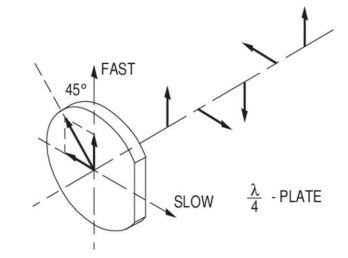
\includegraphics[height=4cm, width=6.3cm]{OPT0.png}
				\caption{\textbf{Quarter wave Plate turning linear polarizationg to circular polarization}}
				\label{fig3}
			\end{figure}
		\end{itemize}

	\subsection{Experimental Setup and Apparatus}
		As shown in figure $\ref{fig4}$, the setup consists of a He-Ne laser with power supply that is mounted on a stand and fixed to an optical bench, while a polarizer and an indentical analyzer is placed in line with it on the bench using post holders to allow the unpolarized beam to fall normally on it. The beam is allowed to fall on an affixed photo-detector connected to a digital multimeter which reads a current propotional to the intensity of the falling beam.

		% \vspace{-5mm}
		\begin{figure}[H]
			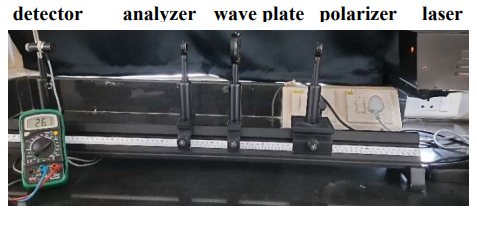
\includegraphics[height=3.5cm, width=9cm]{OPT10000.png}
			\caption{\textbf{Experimental Setup}}
			\label{fig4}
		\end{figure}
	
	% \vspace{-1cm}
